\documentclass{article}
\usepackage[utf8]{inputenc}
\usepackage[english]{babel}

\usepackage{graphicx}
\usepackage{float}
\graphicspath{{figures/}}

\usepackage{todonotes}
\let\oldtodo\todo
\renewcommand{\todo}[1]{\oldtodo[noline]{#1}}

\usepackage{amsmath}
\usepackage{amssymb}
\usepackage{commath}
\newcommand{\RR}{\mathbb{R}}
\newcommand{\NN}{\mathbb{N}}
\newcommand{\ZZ}{\mathbb{Z}}
\newcommand{\T}[1]{#1^{\top}}
\newcommand{\kth}[2][k]{#2^{(#1)}}
\DeclareMathOperator{\diag}{diag}

\usepackage{tocloft}
\setcounter{tocdepth}{4}
\cftsetindents{paragraph}{2ex}{2ex}

\title{Summary of OCS Slides}
\author{Philipp Gabler}
\date{}

\begin{document}
\maketitle

\tableofcontents

%%%%%%%%%%%%%%%%%%%%%%%%%%%%%%%%%%%%%%%%%%%%%%%%%%%%%%%%%%%%%%%%%%
\section{Introduction}

\paragraph{General Form.} A general minimization problem has the form
\begin{equation*}
  \min_{x} f(x) \quad \text{s.t. } x \in X,
\end{equation*}
for a \emph{constraint set} \(X \subseteq \RR^n\) (often given by some \emph{constraint functions}
and an \emph{objective function} \(f: X \to \RR\).  We want to find an optimal value or
\emph{minimizer} \(x^* \in X\) such that
\begin{equation*}
  f(x^*) \leq f(x), \quad \forall x \in X.
\end{equation*}

\paragraph{Types of Optimization Problems.}
\begin{enumerate}
\item
  \begin{enumerate}
  \item Discrete: \(X\) is a discrete set, also called \emph{interger programming}.
  \item Continuous: \(X\) is continuous (ie. uncountable)
  \end{enumerate}
\item
  \begin{enumerate}
  \item Linear: Objective functions and constraints are all linear:
    \begin{equation*}
      \min_x \T{c} x, \quad\text{s.t. } Ax \leq b,\; x \geq 0.
    \end{equation*}
    Constraints describe a polyhedron.  Efficiently solvable.
  \item Quadratic: Objective function is quadratic, constraints linear:
    \begin{equation*}
      \min_x \frac{1}{2}\T{x} Q x + \T{c} x, \quad\text{s.t. } Ax \leq b,\; Ex = d.
    \end{equation*}
    If \(Q\) is positive semidefinite, the objective is convex and the problem is polynomially
    solvable.
  \item Nonlinear: no further constraints.
  \end{enumerate}
\item
  \begin{enumerate}
  \item Unconstrained: Optimal solution searched in full \(\RR^n\). Easier to characterize, and
    usually to solve.
  \item Constrained: Optimal solution in an admissible region, usually more difficult to
    setup/characterize.
  \end{enumerate}
\end{enumerate}

\paragraph{Convexity.}
A set \(X\) is convex, if for all \(x, y \in X\) and \(\alpha \in [0,1]\):
\begin{equation*}
  \alpha x + (1 - \alpha) y \in X.
\end{equation*}
This means that \(X\) contains all convex combinations of points from it.

\paragraph{Convex Functions.}
If \(X\) is a convex set, then \(f: \RR \to \RR\) is called convex if for all \(x, y \in X\) and
\(\alpha \in [0,1]\):
\begin{equation*}
  f(\alpha x + (1 - \alpha) y) \leq \alpha f(x) + (1 - \alpha) f(y).
\end{equation*}
This means that no points lie below any tangent.

\paragraph{Level Sets.}
For an objective function \(f: X \to \RR\), and \(c \in \RR\), the sets
\begin{equation*}
  S_c(f) = \{x \in X: f(x) = c\}
\end{equation*}
are called \emph{level sets} of \(f\). They can be convex even if \(f\) is not!

\paragraph{Definiteness.}
A matrix \(Q\) is called \emph{positive semidefinite} if \(\T{x} Q x \geq 0\) for all \(x\).  \(Q\)
is called \emph{positive definite} if \(\T{x} Q x > 0\) for all \(x \neq 0\).  Sometimes this is
written as \(Q \succeq 0\) and \(Q \succ 0\).

\paragraph{Local and Global Minima.}
A point \(x^*\) is called an \emph{unconstrained global minimum} of \(f\) if for all \(x\)
\begin{equation*}
  f(x^*) \leq f(x).
\end{equation*}
\(x^*\) is called an \emph{unconstrained local minimum} of \(f\) if it is minimal in some
neighbourhood; i.e., there is an \(\epsilon > 0\) such that
\begin{equation*}
  f(x^*) \leq f(x) \quad \forall x \text{ with } \lVert x^* - x \rVert \leq \epsilon.
\end{equation*}
For \emph{constrained} minima, we just require additionally that \(x \in X \subset \RR^n\).

\paragraph{First Order Neccessary Condition for Optimality.}
In a small neighbourhood of \(x^*\), we can by Taylor expansion write \(f\) as
\begin{equation*}
  f(x) = f(x^* + \Delta x) = f(x^*) + \T{\nabla f(x^*)} \Delta x + o(\lVert \Delta x \rVert).
\end{equation*}
Since \(x^*\) is a local minimum, \(f(x^* + \Delta x) - f(x^*) \geq 0\), and we have
\begin{equation*}
  f(x^*) + \T{\nabla f(x^*)} \Delta x - f(x^*) = \T{\nabla f(x^*)} \Delta x \geq 0.
\end{equation*}
Since wlog. we can choose \(\Delta x\) to have the opposite sign, it holds also that
\begin{equation*}
  \T{\nabla f(x^*)} \Delta x \leq 0,
\end{equation*}
so \(\T{\nabla f(x^*)} \Delta x = 0\), which, since \(\Delta x\) is arbitrary, implies that
\(\nabla f(x^*) = 0\).

\paragraph{Second Order Neccessary Condition for Optimality.}
By second order Taylor expansion, we get
\begin{align*}
  0 &\leq f(x^* + \Delta x) - f(x^*) \\
    &= f(x^*) + \underbrace{\T{\nabla f(x^*)} \Delta x}_{= 0} +
      \frac{1}{2} \T{\Delta x} \nabla^2 f(x^*) \Delta x + o(\lVert \Delta x \rVert^2) - f(x^*) \\
    &=  \frac{1}{2} \T{\Delta x} \nabla^2 f(x^*) \Delta x + o(\lVert \Delta x \rVert^2).
\end{align*}
From this follows that \(\T{\Delta x} \nabla^2 f(x^*) \Delta x \geq 0\).  Since \(\Delta x\) is
arbitrary, this means that \(\nabla^2 f(x^*)\) must be positive semidefinite.

A point which has this property is called a \emph{stationary point}.  In ``normal'' cases, it is
either a local optimum or a saddle point.

\paragraph{Sufficient Condition for Optimality.}
If for a point \(x^*\) we have \(\T{\nabla f(x^*)} = 0\) and \(\nabla^2 f(x^*)\) positive
\emph{definite} (no ``semi-''!), then \(x^*\) is a strict unconstrained local minimum of
f. 

\paragraph{Minima of Convex Functions.}
For a convex function \(f\), local minima are also global minima: suppose \(x*\) were a local, but
not global minimum. Then there must be some \(y^* \neq x^*\) with \(f(y^*) < f(x^*)\).  By
convexity, we have for all \(\alpha \in [0, 1)\):
\begin{equation*}
  f(\alpha x^* + (1 - \alpha) y^*) < \alpha f(x^*) + (1 - \alpha) f(y^*) < f(x^*),
\end{equation*}
which contradicts the assumption, so \(x^*\) must also be a global minimum.

Furthermore, the neccessary condition for minima, \(\nabla f(x^*) = 0\), for convex functions
becomes a sufficient condition.\todo{why this?}

%%%%%%%%%%%%%%%%%%%%%%%%%%%%%%%%%%%%%%%%%%%%%%%%%%%%%%%%%%%%%%%%%%
\section{Gradient Methods}

\paragraph{Basic Idea.}
To find a minimum of \(f\), we construct a sequence \(\kth{x}\) such that for all \(k\),
\(f(\kth[k+1]{x}) < f(\kth{x})\).  To do that, we choose an initial \(\kth[0]{x}\) and then set
\begin{equation*}
  \kth[k+1]{x} = \kth{x} + \kth{\alpha} \kth{d}.
\end{equation*}
Here \(\kth{\alpha}\) is some step size, and \(\kth{d}\) is a \emph{descent direction} which must
satisfy
\begin{equation*}
  \pd{f}{{\kth{d}}}(\kth{x}) = \T{\nabla f(\kth{x})} \kth{d} < 0, 
\end{equation*}
where \(\pd{f}{{\kth{d}}}\) is the directional derivative in direction \(\kth{d}\).

\paragraph{Matrix-Scaled Gradients.}
Given the above form, one can choose \(\kth{d} = -\kth{D} \nabla f(\kth{x})\) for a positive
definite \(\kth{D}\):
\begin{equation*}
  \T{\nabla f(\kth{x})} \kth{d} = -\T{\nabla f(\kth{x})} \kth{D} \nabla f(\kth{x}) < 0,
\end{equation*}
by the definition of positive definiteness.

\begin{enumerate}
\item Steepest descent: \(\kth{D} = I\). Simple, but slow convergence.
\item Newton's method: \(\kth{D} = (\nabla^2 f(\kth{x}))^{-1}\).  Fast convergence, but
\(\nabla^2 f(\kth{x})\) needs to be positive definite to be invertible.  Corresponds to local
approximation by a quadratic surface (see below). \todo{references to later sections}
\item Levenberg-Marquart method: \(\kth{D} = (\nabla^2 f(\kth{x}) + \lambda I)^{-1}\).  Tries
to fix problems with Newton's method by regularization.
\item Diagonal scaling: \(\kth{D} = \diag(\kth{d}_1, \ldots, \kth{d}_n)\). E.g. approximating
Newton's method with
\begin{equation*}
  \kth{d}_i = \left( \pd[2]{f}{x_i}(\kth{x}) \right)^{-1}.
\end{equation*}
\item Gauss-Newton method: For a nonlinear least-squares problem
\(f(x) = \frac{1}{2} \lVert g(x) \rVert^2\), we can choose
\(\kth{D} = ( \nabla g(\kth{x} \T{\nabla g(\kth{x})})^{-1}\).  This is related to the
pseudo-inverse.
\end{enumerate}

\paragraph{Step Size Selection.}
To ensure convergence and performance, \(\kth{\alpha}\) needs to be chosen with care.
Theoretically, it is not enough set it such that \(f(\kth[k+1]{x}) < f(\kth{x})\); there are
counterexamples for which this holds, but \(\lim_{, \to \infty} f(\kth{x}) > f(x^*)\), e.g., when
the step sequence in the limit oscillates between two values on the opposite sides of a ``bowl''.

Some usual approaches to choosing the step size are:
\begin{enumerate}
\item Minimization rule: choose \(\kth{\alpha}\) such that the minimum in the descent direction is
  taken, i.e.
  \begin{equation*}
    f(\kth{x} + \kth{\alpha}\kth{d}) = \min_{\alpha \geq 0} f(\kth{x} + \alpha\kth{d}).
  \end{equation*}
\item Limited minimization rule: ``heuristically'' search the best \(\kth{\alpha}\) in some set,
  like in an interval \([0, s]\) or among some values \(\{\beta^0 s, \beta^1 s, \ldots \}\) for some
  fixed \(\beta \in (0, 1)\) and \(s > 0\).
\item Constant step size: sometimes, an optimal (or good enough) value \(\kth{\alpha} = s\) can be
  computed from the objective function in advance.
\item Diminishing step size: choose a decreasing sequence with
  \(\lim_{k \to \infty} \kth{\alpha} = 0\) and \(\sum_{k = 0}^{\infty} \kth{\alpha} = \infty\).  The
  latter is sufficient to ensure convergence (we can never ``run out of space'' before the optimum
  is reached).  This has good theoretical properties for some setups, but the convergence rate can
  be quite slow.
\end{enumerate}

\paragraph{Armijo Rule.}
This is a special method for step size selection, which has nice theoretical properties (e.g. using
it, the \(\kth{x}\) always converge to a stationary point).  To apply it, we fix scalars \(s\), \(0 <
\beta < 1\), and \(0 < \sigma < 1\), and set \(\kth{\alpha} = \beta^{m_k} s\), where we choose
\(m_k\) as the first nonnegative integer for which
\begin{equation*}
  f(\kth{x} + \beta^{m_k} s \kth{d}) - f(\kth{x}) \leq \sigma \beta^{m_k} s \nabla \T{f(\kth{x})} \kth{d}.
\end{equation*}

The interpretation of this is that we try out the step sizes \(\beta^{m_k} s\) in decreasing order,
until we find one for which the decrease in the objective is sufficiently large.

\begin{figure}[H]
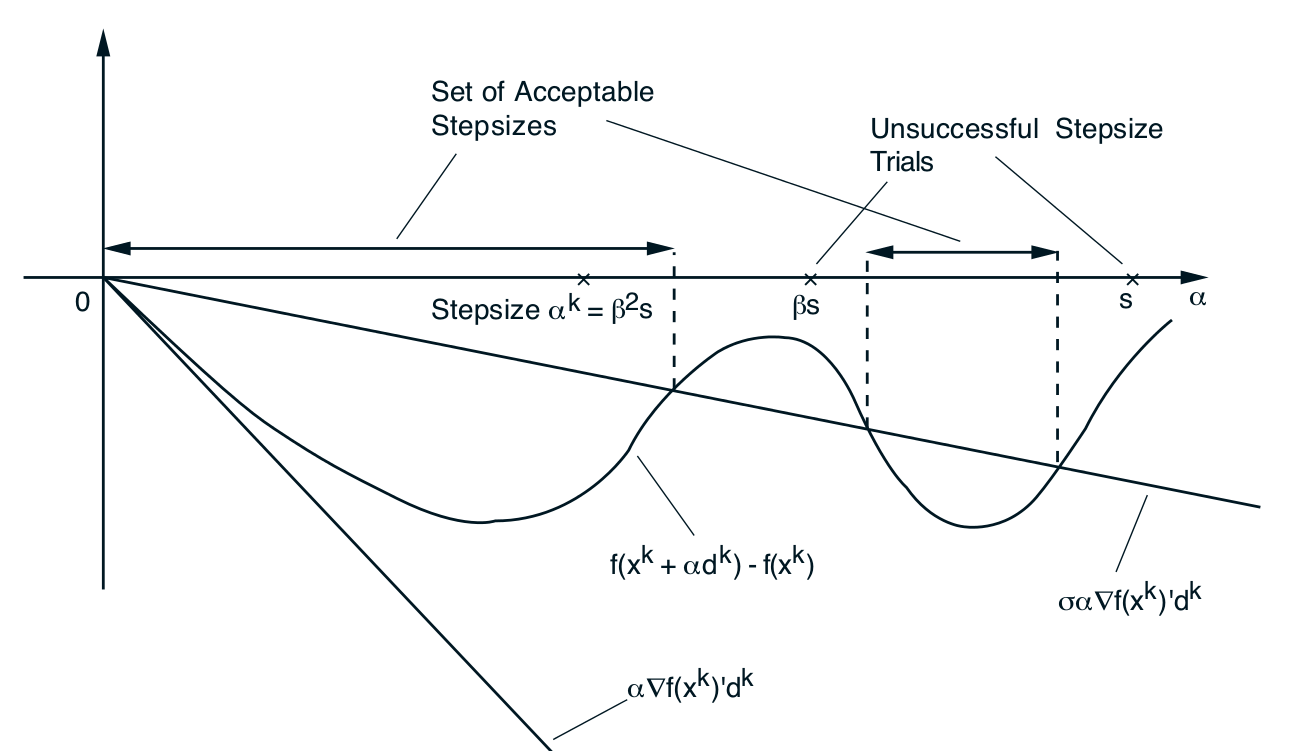
\includegraphics[width=\textwidth]{armijo.png}
\caption{Graphical interpretation of Armijo rule.\label{fig:armijo}}
\end{figure}

\paragraph{Termination of Gradient Methods.}
Gradient methods are not automatically convergent, so we need some stopping criterion.  The standard
approach is to terminate iteration based on the norm of the gradient:
\begin{equation*}
  \lVert \nabla f(\kth{x}) \rVert \leq \epsilon,
\end{equation*}
for some reasonable \(\epsilon > 0\).  Since the absolute sizes of the gradients are not
neccessarily meaningful, a better criterion is
\begin{equation*}
  \frac{\lVert \nabla f(\kth{x}) \rVert}{\lVert \nabla f(\kth[0]{x}) \rVert} \leq \epsilon.
\end{equation*}
Assuming we have diagonal scaling, we can also use
\(\lVert \kth{D} \nabla f(\kth[0]{x}) \rVert \leq \epsilon\).

If \(\nabla^2 f(x)\) is positive definite, we have a strongly convex problem, and the norm of the
gradient actually bounds the distance to a local minimum \(\lVert x - x^* \rVert\).


\end{document}
